\documentclass{standalone}
% translate with >> pdflatex -shell-escape <file>

% This file is an extract of the PGFPLOTS manual, copyright by Christian Feuersaenger.
% 
% Feel free to use it as long as you cite the pgfplots manual properly.
%
% See
%   http://pgfplots.sourceforge.net/pgfplots.pdf
% for the complete manual.
%
% Any required input files (for <plot table> or <plot file> or the table package) can be downloaded
% at
% http://www.ctan.org/tex-archive/graphics/pgf/contrib/pgfplots/doc/latex/
% and
% http://www.ctan.org/tex-archive/graphics/pgf/contrib/pgfplots/doc/latex/plotdata/

\usepackage{pgfplots}
\usepackage{pgfplotstable}
\pgfplotsset{compat=newest}

% The manual loads these libraries globally; the extracted standalone examples
% need them too. external/clickable/snakes are intentionally omitted.
\usetikzlibrary{
	arrows.meta,backgrounds,calc,decorations.footprints,decorations.markings,
	decorations.pathreplacing,fixedpointarithmetic,intersections,patterns,
	plotmarks,shapes.arrows,spy,through}
\usepgfplotslibrary{
	colorbrewer,colormaps,dateplot,fillbetween,groupplots,patchplots,polar,
	smithchart,statistics,ternary,units}

% Some colormap examples reuse this display style defined earlier in the manual.
\pgfplotsset{
	cycle from colormap manual style/.style={
		x=3cm,y=10pt,ytick=\empty,
		colorbar style={x=,y=,ytick=\empty},
		point meta min=0,point meta max=1,
		stack plots=y,
		y dir=reverse,colorbar style={y dir=reverse},
		every axis plot/.style={line width=2pt},
		legend entries={0,...,20},
		legend pos=outer north east,
	},
}

\pagestyle{empty}
\usetikzlibrary{patterns}

\begin{document}
% \usetikzlibrary{patterns}
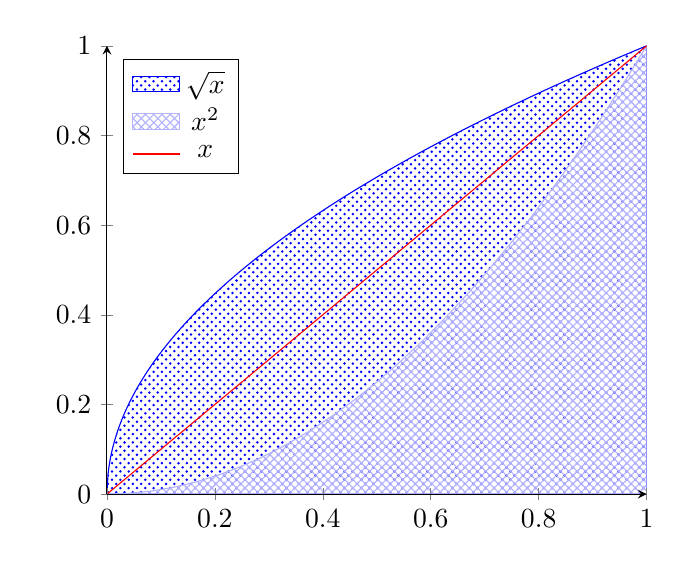
\begin{tikzpicture}
\begin{axis}[area legend,
    axis x line=bottom,axis y line=left,
    domain=0:1,
    legend pos=north west,
    axis on top,xmin=0,
]
    \addplot [pattern=crosshatch dots,
        pattern color=blue,draw=blue,
        samples=500]
            {sqrt(x)} \closedcycle;
    \addplot [pattern=crosshatch,
        pattern color=blue!30!white,
        draw=blue!30!white]
            {x^2}     \closedcycle;
    \addplot [red,line legend]
        coordinates {(0,0) (1,1)};
    \legend{$\sqrt x$,$x^2$,$x$}
\end{axis}
\end{tikzpicture}
\end{document}
